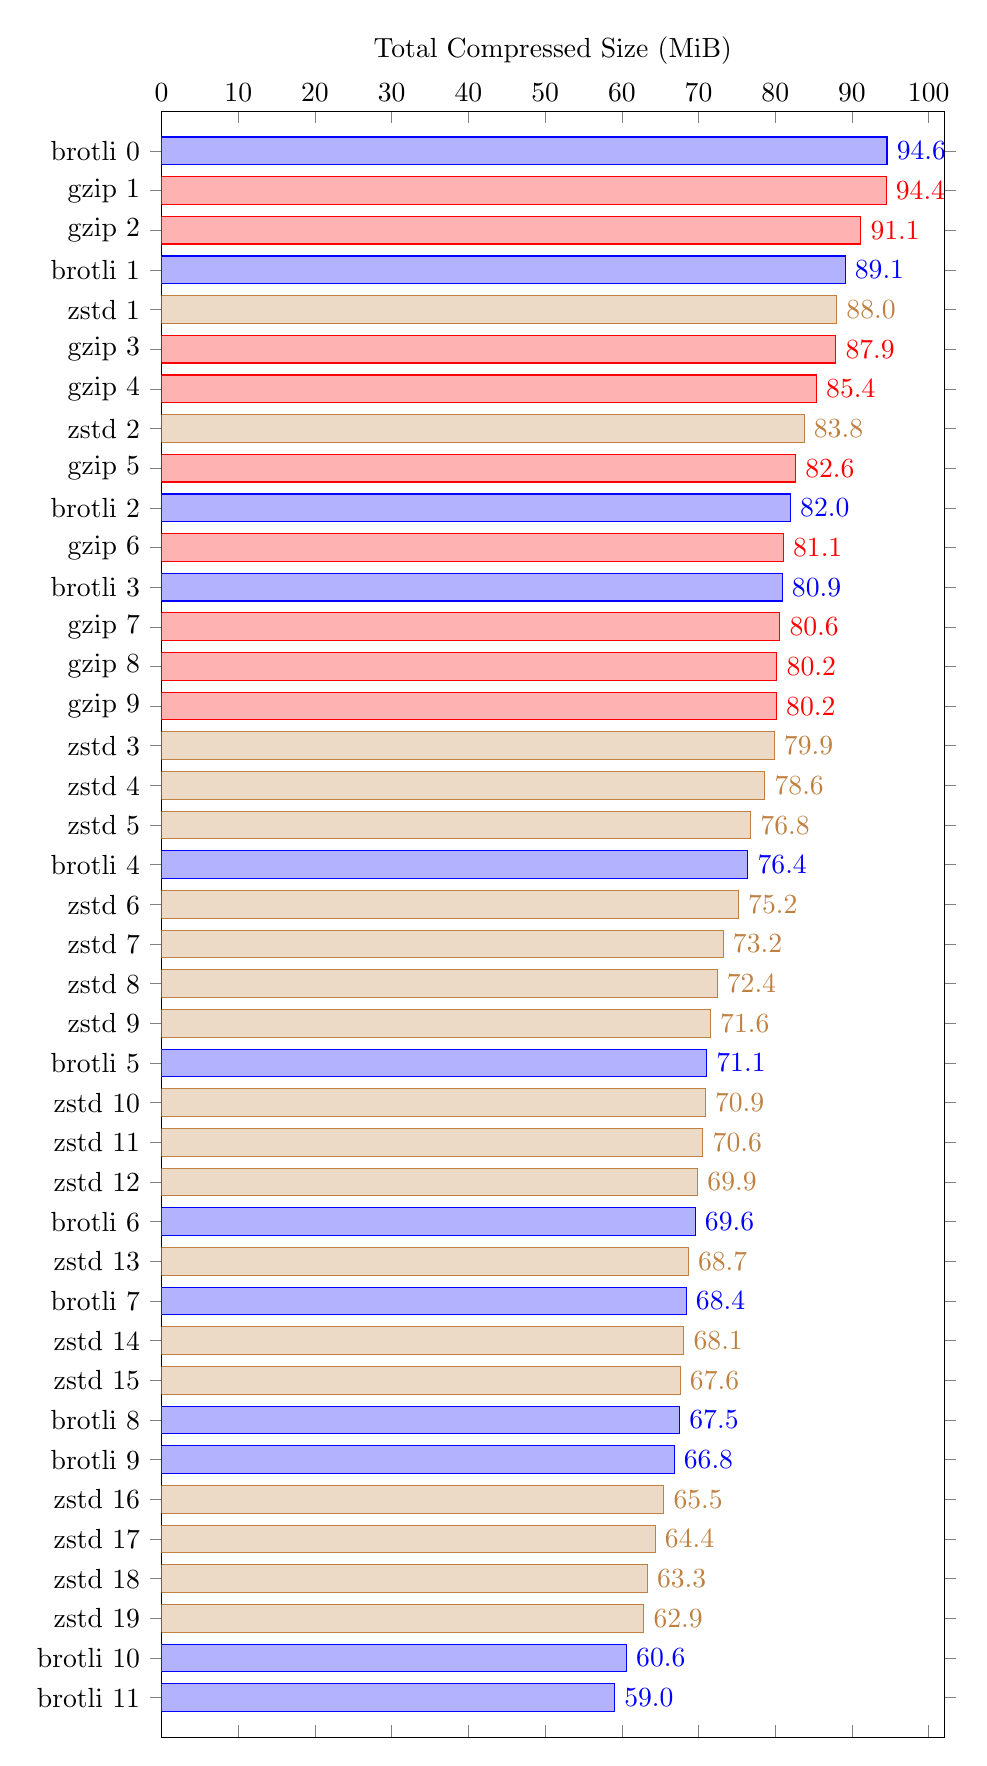
\begin{tikzpicture}
\begin{axis}[
	width = 0.95*\textwidth,
	height = 3.056*\axisdefaultheight,
	xbar,
	xmin = 0,
	xmax = 102,
	xtick = {0, 10, 20, 30, 40, 50, 60, 70, 80, 90, 100},
	xticklabel pos = right,
	y dir = reverse,
	ytick = {
		0, 1, 2, 3, 4, 5, 6, 7, 8, 9, 10,
		11, 12, 13, 14, 15, 16, 17, 18, 19, 20,
		21, 22, 23, 24, 25, 26, 27, 28, 29, 30,
		31, 32, 33, 34, 35, 36, 37, 38, 39
	},
	yticklabels = {
		brotli 0,
		gzip 1,
		gzip 2,
		brotli 1,
		zstd 1,
		gzip 3,
		gzip 4,
		zstd 2,
		gzip 5,
		brotli 2,
		gzip 6,
		brotli 3,
		gzip 7,
		gzip 8,
		gzip 9,
		zstd 3,
		zstd 4,
		zstd 5,
		brotli 4,
		zstd 6,
		zstd 7,
		zstd 8,
		zstd 9,
		brotli 5,
		zstd 10,
		zstd 11,
		zstd 12,
		brotli 6,
		zstd 13,
		brotli 7,
		zstd 14,
		zstd 15,
		brotli 8,
		brotli 9,
		zstd 16,
		zstd 17,
		zstd 18,
		zstd 19,
		brotli 10,
		brotli 11
	},
	scaled ticks = false,
	enlarge x limits = {abs = 0},
	enlarge y limits = {abs = 1},
	nodes near coords,
	nodes near coords align = {horizontal},
	nodes near coords style = {/pgf/number format/.cd, fixed zerofill, precision = 1},
	every axis plot/.append style = {xbar, fill, bar shift = 0pt},
	xlabel near ticks,
	xlabel = Total Compressed Size (MiB)
]
\addplot[blue, fill = blue!30!white] coordinates {
	(94.56, 0)  % 99 150 297 B
	(89.10, 3)  % 93 429 734 B
	(81.98, 9)  % 85 960 725 B
	(80.90, 11) % 84 830 319 B
	(76.42, 18) % 80 136 146 B
	(71.05, 23) % 74 500 236 B
	(69.56, 27) % 72 940 373 B
	(68.39, 29) % 71 711 758 B
	(67.53, 32) % 70 807 826 B
	(66.81, 33) % 70 055 213 B
	(60.60, 38) % 63 543 079 B
	(59.04, 39) % 61 911 912 B
};
\addplot[red, fill = red!30!white] coordinates {
	(94.44, 1)  % 99 027 630 B
	(91.14, 2)  % 95 567 413 B
	(87.88, 5)  % 92 146 479 B
	(85.36, 6)  % 89 507 810 B
	(82.64, 8)  % 86 656 402 B
	(81.05, 10) % 84 987 646 B
	(80.58, 12) % 84 495 896 B
	(80.21, 13) % 84 110 750 B
	(80.15, 14) % 84 047 624 B
};
\addplot[brown, fill = brown!30!white] coordinates {
	(88.00, 4) % 92 275 340 B
	(83.76, 7) % 87 832 541 B
	(79.86, 15) % 83 737 813 B
	(78.64, 16) % 82 460 802 B
	(76.79, 17) % 80 524 085 B
	(75.20, 19) % 78 852 204 B
	(73.21, 20) % 76 761 040 B
	(72.41, 21) % 75 927 488 B
	(71.55, 22) % 75 027 107 B
	(70.87, 24) % 74 314 109 B
	(70.57, 25) % 74 002 318 B
	(69.88, 26) % 73 270 742 B
	(68.66, 28) % 71 991 701 B
	(68.08, 30) % 71 391 788 B
	(67.60, 31) % 70 888 796 B
	(65.46, 34) % 68 641 121 B
	(64.35, 35) % 67 480 010 B
	(63.31, 36) % 66 383 640 B
	(62.86, 37) % 65 912 429 B
};
\end{axis}
\end{tikzpicture}